\chapter{An Overview on Software Product Lines, Requirements Engineering, SPL
Requirements Engineering and SPL Tools}
\label{ch:background}


This chapter presents fundamental information for the understanding of four
topics that are relevant to this work: software product lines, requirements
engineering, and \ac{SPL} requirements engineering. \secref{sc:productlines} discusses the
motivation, benefits, and the SPL development process.
\secref{sc:requirementsengineering} presents requirements engineering.
\secref{sc:splrequirementsengineering} presents \ac{SPL} requirements engineering.
\secref{sc:spltools} presents \ac{SPL} Tools. Finally, \secref{sc:summary} presents a
summary of this chapter.


\section{Software Product Lines}
\label{sc:productlines}

\subsection{Introduction}
Nowadays we experience the age of customization, but it was not always like
that. There was a time when goods were handcrafted for individual costumers. 
Over the years, the number of people who could afford to buy several kinds of 
products has increased \citep{Pohl2005}. In order to meet this rising demand, 
the production line was invented, which enabled production for a mass market much 
more cheaply than individual product.

Customers were satisfied with mass produced products for a while \citep{Pohl2005}, 
however that kind of product lacks sufficient diversification to meet individual
customers’ wishes. Individualized products also have a drawback; they are a lot more expensive 
than standardized products. In that context, the industry was challenged to provide customized 
products at reasonable costs to satisfy the wishes of specific customers and market segments. 
The combination of mass customization and common platforms was the key to achieve that goal.

Mass customization is the large-scale production of goods tailored to individual
customers’ needs. It requires a higher technological investment which leads to higher prices for 
the individualized products and/or to lower profit margins for the company. The platform approach 
though, enables manufacturers to offer a larger variety of products and to reduce costs at the same 
time. A platform is defined as a base of technologies on which other technologies or processes are 
built. The combination of mass customization and a common platform allows us to reuse a common 
base of technology and to bring out products in close accordance with customers’ wishes \citep{Pohl2005}.

In the software domain, that combination resulted in a software development
paradigm called \acf{SPLE}. A Software
Product Line (\ac{SPL}) is a set of software-intensive systems that share a common, managed feature set, satisfying a particular market 
segment’s specific needs or mission and that are developed from a common set of core assets in a 
prescribed way \citep{clements2002software}.

\subsection{The Benefits}
Developing software under the Product Line Engineering paradigm offers many benefits for a company, 
some examples follow:
\begin{itemize}
\item \textbf{Reduction of Development Costs}

A good reason for applying the Product Line Engineering paradigm is the reduction of costs as the reuse 
of assets increases. Through the reuse of artifacts from the platform in different systems, the development 
of each of these systems becomes cheaper. First, the company has to invest in the development of the platform. 
Also, the way in which the artefacts from the platform will be reused has to be well planned beforehand. Then, 
from a certain point, called break-even point, the initial investment will be paid off. The precise location of 
this point is influenced by many characteristics of the company, the market it has envisaged, its customers, 
expertise, kinds of products, the way the product line is created and others. 

\begin{figure}[htp]
\begin{center}
  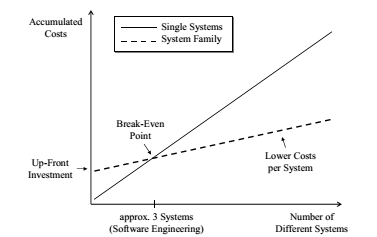
\includegraphics[width=11cm]{chapters/background/img/splcosts.png}
  \caption[Costs for developing systems as single systems compared to product 
  line engineering]{Costs for developing systems as single systems compared to product line engineering \citep{Pohl2005}}
  \label{fg:spl-costs}
\end{center}
\end{figure}

\figref{fg:spl-costs} shows that the costs to develop a few systems in an \ac{SPL} approach are higher than in a 
single systems approach. However, using product line engineering, the costs are significantly lower for larger 
systems quantities. 

\item \textbf{Quality improvement}

Creating products under the \ac{SPL} paradigm improves the quality of all products of a product family. 
The shared components from the platform are reviewed and tested in many products. They have to work properly in 
more than one kind of product. The extensive quality assurance indicates a significantly higher opportunity of 
detecting faults and correcting them, thereby improving the quality of all products \citep{Pohl2005}.

\begin{figure}[htp]
\begin{center}
  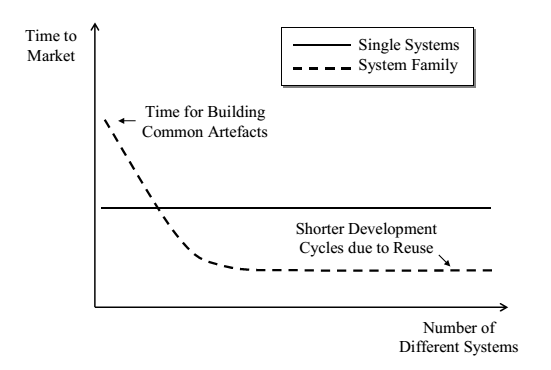
\includegraphics[width=11cm]{chapters/background/img/spl-timetomarket.png}
  \caption[Comparison of time to market with and without product line
  engineering]{Comparison of time to market with and without product line
  engineering \citep{Pohl2005}}
  \label{fg:spl-timetomarket}
\end{center}
\end{figure}

\item \textbf{Reduction of Time-to-market}

Another very important success factor for a product is the time to market.
\ac{SPL} engineering demands a high upfront investment, which makes time to
market initially higher if compared with to single-systems engineering. However, as the reuse of artefacts grow, 
the time to market is significantly shortened for new products, as can be seen
in \figref{fg:spl-timetomarket}.
\item \textbf{Reduction of Maintenace Effort}

When a reusable asset from the platform is changed, this change may be
propagated to all products in which it is being used. It usually leads to a simpler and cheaper maintenance and 
evolution, if compared to maintain and evolve a bunch of single products in a separate way.

\item \textbf{Benefits for the Customers}

The benefits for the customers are higher quality products at reasonable prices
because the production costs become lower in \ac{SPL} engineering. Besides, products are adapted to their 
real needs and wishes.
\end{itemize}


\subsection{The SPL Development Process}
There are a number of different definitions for the \acf{SPL} Development
Process on the literature. \citep{Pohl2005} introduced a framework for SPLE paradigm, shown in
\figref{fg:spl-pohlframework}. This framework is divided in two processes: 

\begin{figure}[htp]
\begin{center}
  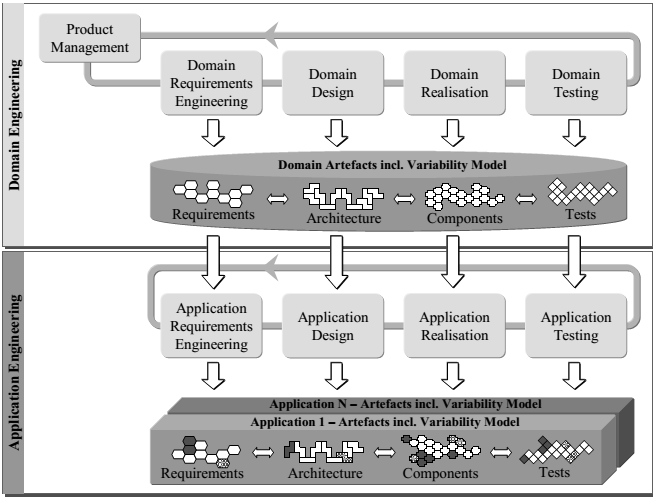
\includegraphics[width=13cm]{chapters/background/img/pohl-framework.png}
  \caption[The software product line engineering framework]{The software product line engineering framework \citep{Pohl2005}}
  \label{fg:spl-pohlframework}
\end{center}
\end{figure}

\begin{itemize}
\item \textbf{Domain engineering:} This is the process that aims to establish a reusable 
platform and define the commonality and the variability of the product line. Domain Engineering 
is composed of five sub-processes: domain requirements, domain design, domain realization, domain 
testing, and product management \citep{Pohl2005}. 
\item \textbf{Application engineering:} This process is responsible for deriving
product line applications from the platform created in domain engineering, where the previously 
developed components are assembled to compose a product. The application engineering is composed 
of four sub-processes: application requirements engineering, application design, application realization, 
and application test \citep{Pohl2005}.  
\end{itemize}

Another popular  definition of the \acf{SPL} Development
Process  can be related to the aforementioned approach. \citep{clements2002software} 
defined three essential activities to Software Product Lines:
\textbf{\acf{CAD}}, \textbf{\acf{PD}} and \textbf{Management activity},
ilustrated in \figref{fg:spl-activities}.
In essence, \acf{CAD} activity is the Domain engineering process, 
and the \acf{PD} activity is the Application engineering process. 
The main difference between these approaches is the Management activity, which is not considered 
as a process in the first mentioned approach \citep{Pohl2005}. 

\begin{figure}[htp]
\begin{center}
  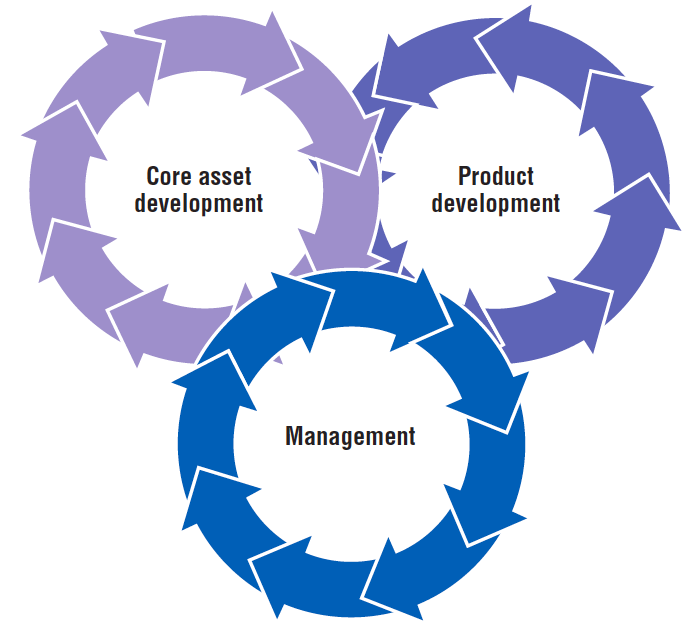
\includegraphics[width=10cm]{chapters/background/img/SPLactivities.png}
  \caption[SPL Activities]{SPL Activities \citep{clements2002software}}
  \label{fg:spl-activities}
\end{center}
\end{figure}

\subsubsection{Core Asset Development (Domain Engineering)}
\acf{CAD}, also called by \citep{Pohl2005} as domain engineering, is an activity 
that aims to develop assets to be further reused in other activities. In \figref{fg:spl-coreasset}, it is shown the core 
asset development activity, which is  interactive, and its inputs and outputs influence each other. The 
inputs of this activity are product constraints; production constraints; architectural styles; design 
patterns; application frameworks; production strategy and preexisting assets. This phase is composed of the 
following sub processes \citep{Pohl2005}:

\begin{itemize}
\item \textbf{Product Management} deals with the economic aspects associated with the software product line and in particular with the market strategy.
\item \textbf{Domain Requirements Engineering} involves all activities for eliciting and documenting the common and variable requirements of the product line.
\item \textbf{Domain Design} encompasses all activities for defining the reference architecture of the product line, 
\item \textbf{Domain Realization} deals with the detailed design and the implementation of reusable software components.
\item \textbf{Domain Testing} is responsible for the validation and verification of reusable components. 
\end{itemize}

\begin{figure}[htp]
\begin{center}
  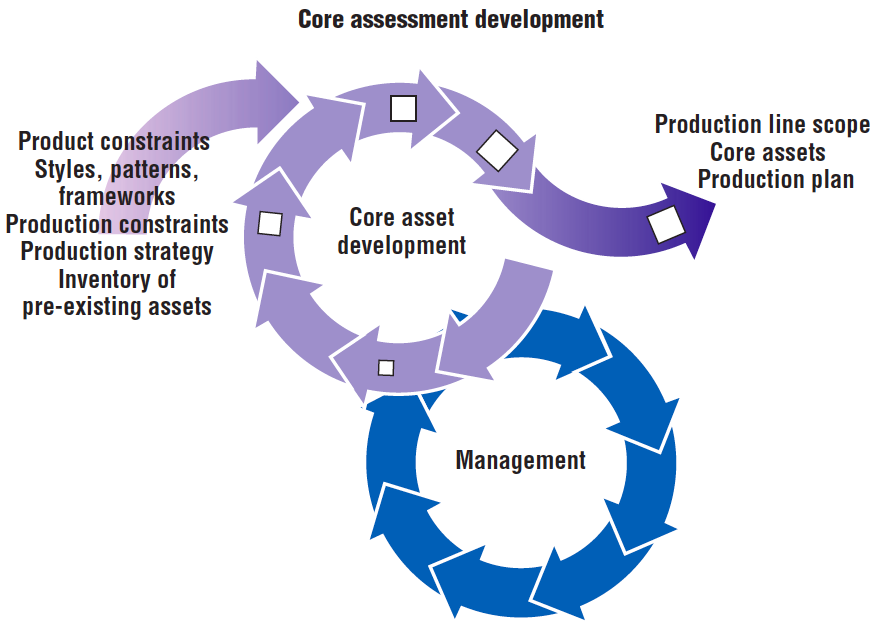
\includegraphics[width=10cm]{chapters/background/img/SPLcoreasserts.png}
  \caption[Core Asset Development]{Core Asset Development \citep{clements2002software}}
  \label{fg:spl-coreasset}
\end{center}
\end{figure}

This activity have three outputs: \textbf{Product Line Scope}, \textbf{Core
Assets} and \textbf{Production Plan}. The Product Line Scope describes the
products that will compose the product line or that the product line can include. This description is recommended to be detailed and well 
specified, for example, including market analysis activities in order to determine the product 
portfolio and to encompass which assets and products will be part of the product line. This 
specification must be driven by economic and business reasons to keep the product line 
competitive \citep{rafael2013systems}. 

Core assets are the basis for production of products in the product line. It
includes an architecture that will fulfill the needs of the product line, specify 
the structure of the products and the set of variation points required to support the 
spectrum of products. It may also include components and their documentation \citep{clements2002software}. 

Lastly, the production plan describes how products are produced from the core
assets. It details the overall scheme of how the individual attached processes can be 
fitted together to build a product \citep{clements2002software}. It is what links all the 
core assets together, guiding the product development within the constraints of the product line.

\subsubsection{Product Development}

\begin{figure}[htp]
\begin{center}
  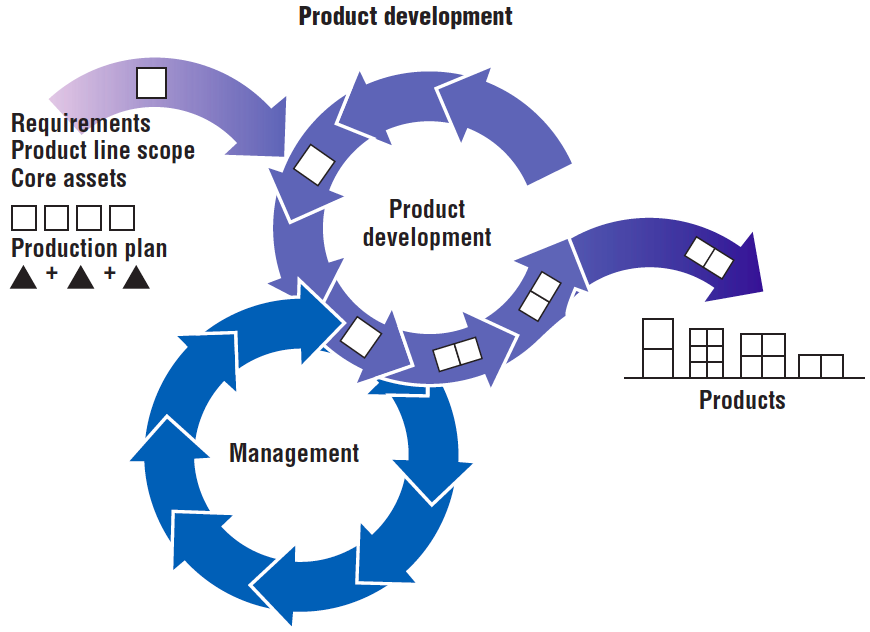
\includegraphics[width=10cm]{chapters/background/img/SPLproduct-development.png}
  \caption[Product Development]{Product Development \citep{clements2002software}}
  \label{fg:spl-productdev}
\end{center}
\end{figure}

The inputs for this activity are the outputs of the core asset development activity (product line scope, 
core assets, and production plan) and the requirements specification for individual products as seen in 
\figref{fg:spl-productdev}. The production plan guides how individual products within a product line are constructed using 
the core assets.

The outputs from this activity should be analyzed by the software engineer and the corrections must be fed 
back to the \acf{CAD} activity. During the product development process, some insights happen 
and it is important to report problems and faults encountered to keep the core asset base healthy.

\subsubsection{Management}

The management activity is responsible for the production strategy and is vital
for success of the product line \citep{Pohl2005}. It is performed in two levels: technical and 
organizational. The technical management supervise the CAD and PD activities by certifying that both 
groups that build core assets and products are focused on the activities they are supposed to, and follow 
the process. The organizational management must ensure that the organizational units receive the right 
resources in sufficient amounts \citep{clements2002software}.

\section{Requirements Engineering}
\label{sc:requirementsengineering}

Software requirements are descriptions of what the system is expected to do, the
services that it must provide and the constraints it must satisfy
\citep{Sommerville2011}.
Software requirements are usually classified in a classic way as functional and non-functional. 
Functional requirements describe what the system must do and non-functional requirements place constraints 
on how these functional requirements are implemented
\citep{sommerville2005integrated}.

According to \citep{sommerville1998requirements},
\acf{RE} is the process by which the  software requirements are defined. They
state that a process is an organized set of activities that transforms inputs to 
outputs. Thus, a complete description of a \ac{RE} process should include what
activities are carried out, the structuring or schedule of these activities, who is responsible for each 
activity and the tools used to support the \ac{RE} activities.   

The \ac{RE} lifecycle includes requirements elicitation, analysis, negotiation, specification, verification, and 
management, where \citep{clements2002software,sommerville2005integrated}:

\begin{itemize}
\item \textbf{Elicitation} identifies sources of requirements information and discovers the 
users’ needs and constraints for the system.
\item \textbf{Analysis} understands the requirements, their overlaps, and their conflicts.
\item \textbf{Negotiation} reaches agreement to satisfy all stakeholders,
solving conflicts that are identified.
\item \textbf{Specification} documents the user’s needs and constraints clearly and precisely.
\item \textbf{Verification} checks if the requirements are complete, correct, consistent, and clear.
\item \textbf{Management} controls the requirements changes that will inevitably arise.
\end{itemize}

\section{SPL Requirements Engineering}
\label{sc:splrequirementsengineering}

Requirements are typical assets in SPL. They are specified in reusable models,
in which commonalities and variabilities are documented explicitly. Thus, these requirements 
can be instantiated and adapted to derive the requirements for an individual
product \citep{cheng2007research}.
During product derivation, for each variant asset, it is decided whether the asset is (or is not) supported by 
the product to be built. When a domain requirement is instantiated, it can be become a concrete product requirement. 
Thus, new products in the SPL will be much simpler to specify, because the requirements are reused and tailored 
\citep{clements2002software}. 

Deciding which products to build depends on business goals, market trends,
technological feasibility, and so on. On the other hand, there are many sources of information 
to be considered and many trade-offs to be made. The SPL requirements must be general enough to support 
reasoning about the scope of the SPL, predicting future changes in requirements and anticipated SPL growth. 

In practice, establishing the requirements for an SPL is an iterative and
incremental effort, covering multiple requirements sources with many feedback loops and validation activities 
(Chastek et al. , 2001). Thus, Requirement Engineering (RE) in SPL has an additional cost. Many SPL requirements 
are complex, interlinked, and divided into common, variable and product-specific requirements (Birk et al. , 2003; 
Oliveira et al. , 2014). Regarding to single systems, RE for SPL has some differences, such as 
(Clements and Northrop, 2002; Pohl et al. , 2005; Thurimella and Bruegge, 2007):

\begin{itemize}
\item \textbf{Elicitation} identifies sources of requirements information and discovers the 
users’ needs and constraints for the system.
\item \textbf{Analysis} understands the requirements, their overlaps, and their conflicts.
\item \textbf{Negotiation} reaches agreement to satisfy all stakeholders,
solving conflicts that are identified.
\item \textbf{Specification} documents the user’s needs and constraints clearly and precisely.
\item \textbf{Verification} checks if the requirements are complete, correct, consistent, and clear.
\item \textbf{Management} controls the requirements changes that will inevitably arise.
\end{itemize}

In SPL, RE also has influence of several stakeholders that participate of the
SPL. Identifying stakeholders that directly influence the RE is essential to define the 
requirements negotiation participants. They are responsible for resolving conflicts and providing information. 

Each stakeholder plays a role with respect to the SPL. Many of the stakeholders
that help to define the requirements also use them. These users have different expectations of 
the outputs of SPL analysis. Some may simply want to confirm that their interests have been represented 
(e.g., marketers, domain expert and analyst domain). Others ( e.g., architects and developers) may want to 
describe proposed functional and non-functional capabilities, and their commonality and variability across 
the SPL, thus, those decisions about architectural solutions and asset construction should be taken into account 
(Chastek et al., 2001).

Several approaches to deal with the definition and specification of functional
requirements in SPL development have been proposed over the last few years. Some approaches specify 
the SPL requirements through features and use cases (Griss et al., 1998; Bayer et al., 1999a; Moon et al., 2005; 
Eriksson et al., 2005; Bonifácio and Borba, 2009; Alférez et al., 2011; Mussbacher et al.,2012; Shaker et al., 2012). 
An SPL functional requirement represented as an use case has at least the following fields: identifier, name, 
description, associated feature(s), pre and post-Conditions, and the Main Success Scenario , as shown in 
Table 2.1. It may also have alternative scenarios, includes/extends relationships, and so on. The feature 
associated to the use case handles the variability within the SPL.

Table 2.1: SPL Use Case Example.

However, the approaches for specifying SPL functional requirements do not propose guide- lines, 
showing step by step how the specification should be done. This lack of guidelines may led to some 
challenges and risks.

\section{SPL Tools}
\label{sc:spltools}

\section{Summary}
\label{sc:summary}
In this chapter, we discussed about important concepts to this work: the area of \acf{SPL}, \acf{CASE} tools and \acf{ALM} tools, including motivations, benefits and definitions. We also made a analysis of features and comparison of tools available in market.

Next chapter presents the \acf{SPLICE}, a web-based, collaborative support for the \ac{SPL} lifecycle steps. It will be discussed the requirements, architecture, implementation and other aspects.

